\documentclass[12pt, a4paper]{article}

\usepackage{array}
\usepackage[portuguese]{babel}
\usepackage{chngpage}
\usepackage{enumitem}
\usepackage{float}
\usepackage[a4paper, margin=2cm]{geometry}
\usepackage{graphicx}
\usepackage{hyperref}
\usepackage{longtable}
\usepackage{lscape}
\usepackage{pdfpages}
\usepackage{setspace}

\makeatletter
\renewcommand\section[1]{
    \newpage
    \thispagestyle{empty}
    \vspace*{\fill}
    \@startsection{section}{1}{\z@}{0px}{50px}{\normalfont\Huge\bfseries}{#1}
    \vspace*{\fill}
    \newpage
}
\makeatother

\newenvironment{condition}{
    \begin{itemize}[wide=0pt]
        \vspace{-0.2cm}
}{
        \vspace{-0.5cm}
    \end{itemize}
}

\newcommand\flow[1]{
    Fluxo normal &
    \singlespacing
    \begin{enumerate}[wide=0pt]
        #1
        \vspace{-0.3cm}
    \end{enumerate} \\ \hline
}

\newcommand\otherflow[3]{
    #1 &
    #2
    \singlespacing
    \begin{enumerate}[wide=0pt]
        #3
        \vspace{-0.3cm}
    \end{enumerate} \\ \hline
}

\newenvironment{usecase}[5]{
    \begin{table}[H]
        \centering
        \begin{tabular}{|>{\centering\arraybackslash\bf}m{3cm}|m{13cm}|}
            \hline
            Caso de uso & \textbf{#1} \\

            \hline
            Descrição & #2 \\

            \hline
            Cenários & #3 \\

            \hline
            Pré-condição &
            \begin{condition}
                #4
            \end{condition} \\

            \hline
            Pós-condição &
            \begin{condition}
                #5
            \end{condition} \\

            \hline
}{
    \end{tabular}
\end{table}
}

\title{\textbf{Desenvolvimento de Sistemas de Software \\ \large Trabalho Prático -- Fase I}}
\date{19 de outubro 2024}
\author{
    Grupo 13 \\
    \url{https://github.com/LEI-DSS/DSS2425-Grupo-13}
}

\begin{document}

\begin{center}
    
\includegraphics[width=0.25\textwidth]{Imagens/Capa/EE-C.eps}
\end{center}

{\let\newpage\relax\maketitle}
\maketitle
\thispagestyle{empty}

\chardef\_=`_
\onehalfspacing
\setlength{\parskip}{\baselineskip}
\setlength{\parindent}{0pt}
\def\arraystretch{1.5}

\vspace{2cm}
\begin{center}
    \begin{tabular}{>{\centering}p{0.25\textwidth}
                    >{\centering}p{0.25\textwidth}
                    >{\centering\arraybackslash}p{0.25\textwidth}}
        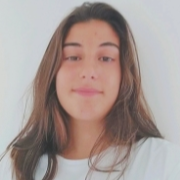
\includegraphics[width=3.5cm]{Imagens/Capa/A104188.png} &
        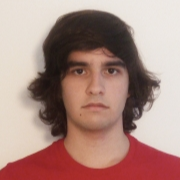
\includegraphics[width=3.5cm]{Imagens/Capa/A104348.png} &
        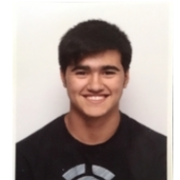
\includegraphics[width=3.5cm]{Imagens/Capa/A95748.png}  \\

        Ana Cerqueira & Humberto Gomes & João Torres \\
        A104188       & A104348        & A95748
    \end{tabular}

    \begin{tabular}{>{\centering}p{0.25\textwidth}
                    >{\centering\arraybackslash}p{0.25\textwidth}}
        
\includegraphics[width=3.5cm]{Imagens/Capa/A104541.png} &
        
\includegraphics[width=3.5cm]{Imagens/Capa/A100612.png} \\

        José Lopes & José Matos \\
        A104541    & A100612
    \end{tabular}
\end{center}

\section{Modelo de Domínio}

\begingroup
    \newgeometry{left=1cm,bottom=1cm,right=1cm,top=1cm}
    \begin{landscape}
        \thispagestyle{empty}

        \begin{figure}
            \centering
            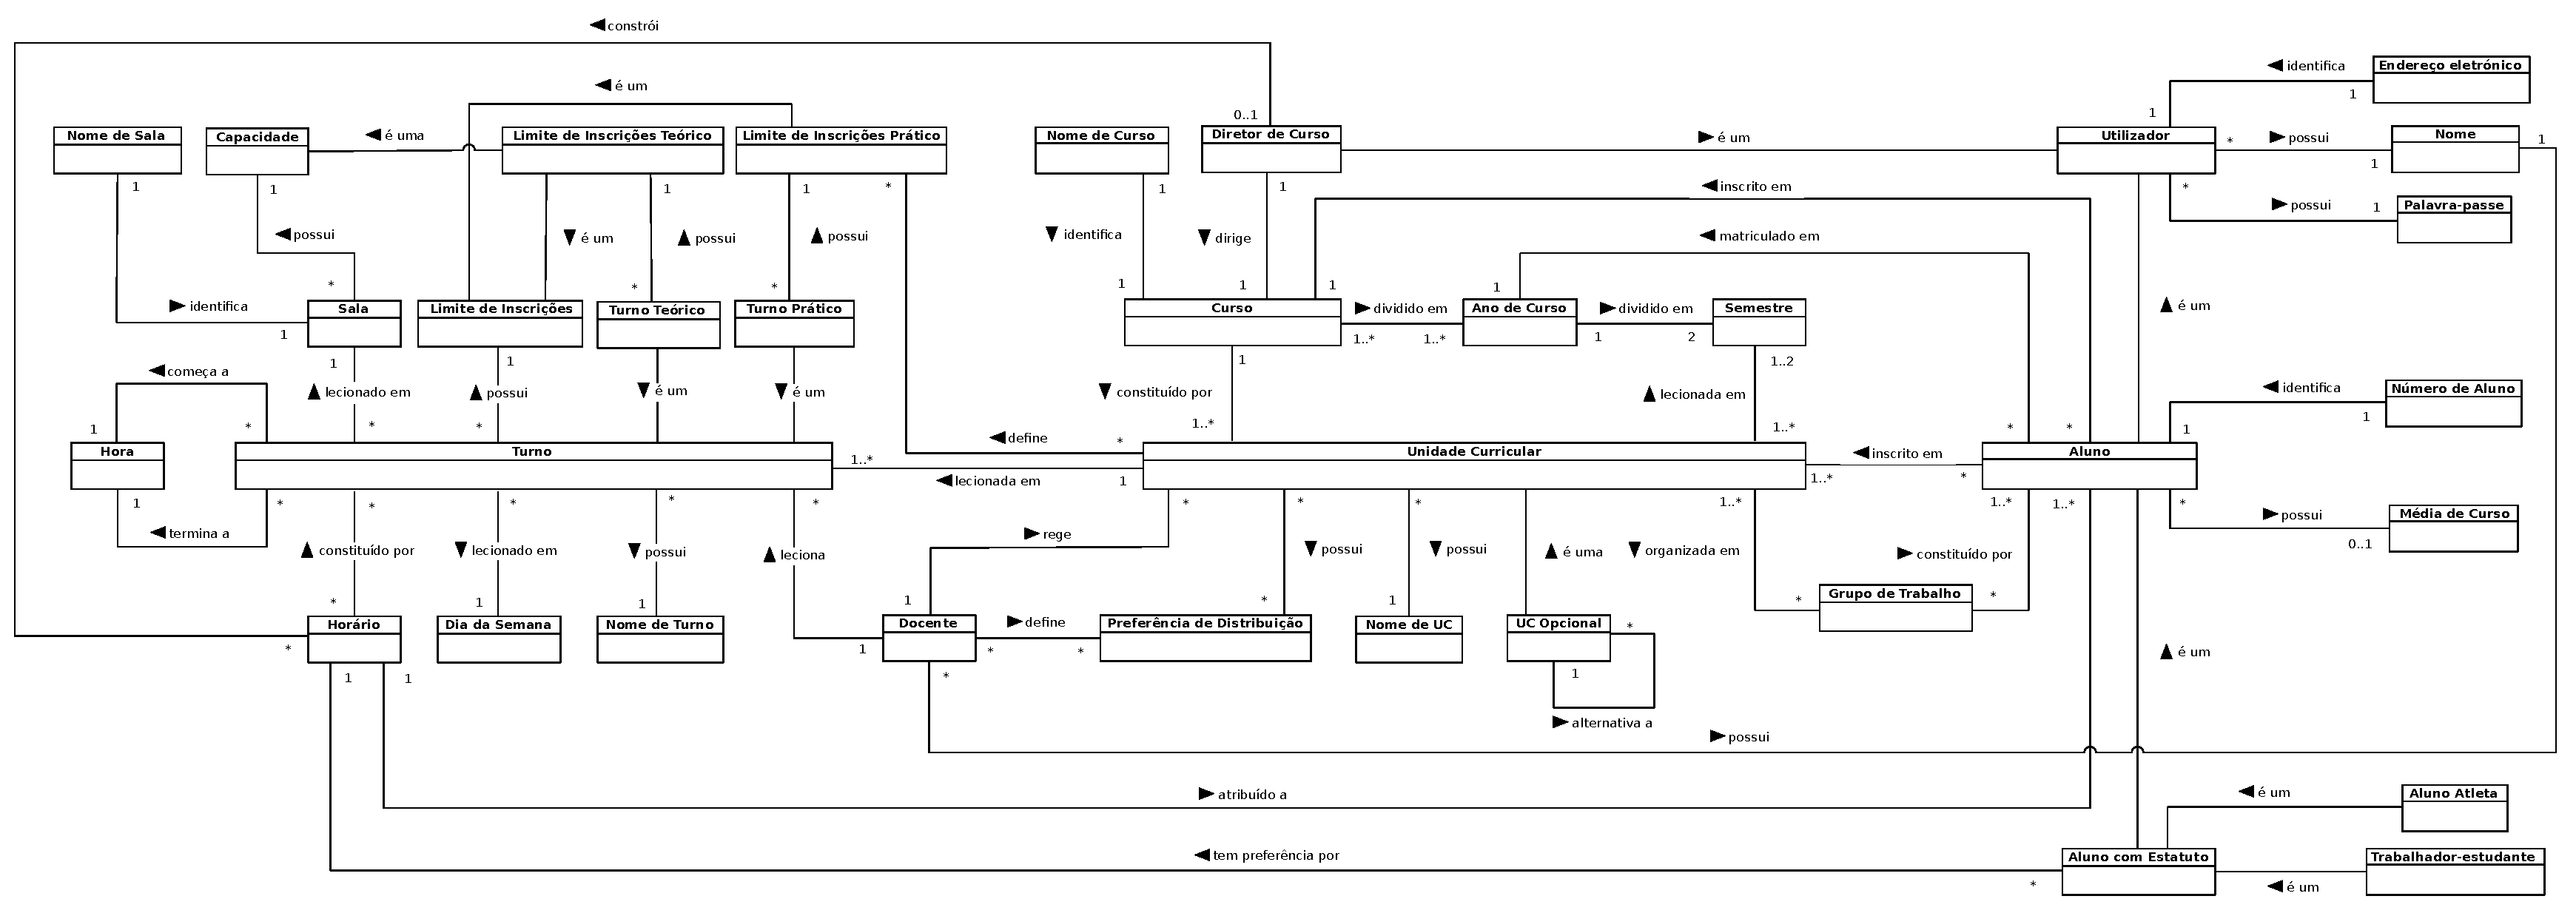
\includegraphics[scale=0.44]{Imagens/Modelos/ModeloDominio.eps}
            \caption{Modelo de Domínio. É recomendado que a sua leitura tenha início na entidade
                Unidade Curricular.}
        \end{figure}
    \end{landscape}
\endgroup

\subsection{Restrições nas relações}

A linguagem de modelação UML não permite expressar restrições nas relações, ou seja, não permite
especificar que dois objetos A e B apenas se podem relacionar caso se verifique uma dada condição,
como, por exemplo, A se relacionar com um outro objeto C. Esta secção do relatório pretende expor
onde, no modelo de domínio construído, se verificam estas situações.

\begin{longtable}{|>{\centering}m{2.5cm}
                  |>{\centering}m{2.5cm}
                  |>{\centering}m{2.5cm}
                  |m{8cm}|}
    \hline
    \textbf{Entidade} & \textbf{Relação} & \textbf{Entidade} & \textbf{Condição necessária} \\
    \hline
    \endfirsthead

    \hline
    \textbf{Entidade} & \textbf{Relação} & \textbf{Entidade} & \textbf{Condição necessária} \\
    \hline
    \endhead

    Aluno              &
    inscrito em        &
    Unidade Curricular &
    Aluno está inscrito no Curso ao qual a Unidade Curricular pertence. \\

    \hline
    Unidade Curricular &
    organizada em      &
    Grupo de Trabalho  &
    Todos os Alunos que constituem o Grupo de Trabalho estão inscritos na Unidade Curricular. \\

    \hline
    Grupo de Trabalho &
    constituído       &
    Aluno             &
    Existe uma Unidade Curricular na qual todos os Alunos que constituem o Grupo de Trabalho se
    encontram inscritos. \\

    \hline
    Aluno          &
    matriculado em &
    Ano de Curso   &
    O Ano de Curso pertence ao conjunto de anos nos quais o Curso em que o Aluno está inscrito se
    divide. \\

    \hline
    Unidade Curricular &
    lecionada em       &
    Semestre           &
    O Curso ao qual a Unidade Curricular pertence contém o Ano de Curso do qual o Semestre faz
    parte. \\

    \hline
    Curso        &
    dividido em  &
    Ano de Curso &
    Existe uma Unidade Curricular do Curso lecionada num Semestre no Ano de Curso. \\

    \hline
    UC Opcional   &
    alternativa a &
    UC Opcional   &
    As duas Unidades Curriculares fazem parte do mesmo Curso. \\

    \hline
    Unidade Curricular          &
    possui                      &
    Preferência de Distribuição &
    A Preferência de Distribuição foi definida pelo Docente que rege a Unidade Curricular. \\

    \hline
    Docente            &
    rege               &
    Unidade Curricular &
    Docente leciona pelo menos um Turno associado à Unidade Curricular. \\

    \hline
    Docente                     &
    define                      &
    Preferência de Distribuição &
    Docente rege pelo menos uma Unidade Curricular. \\

    \hline
    \newpage
    Unidade Curricular           &
    define                       &
    Limite de Inscrições Prático &
    Pelo menos um Turno Prático associado à Unidade Curricular possui o Limite de Inscrições. \\

    \hline
    Turno                &
    possui               &
    Limite de Inscrições &
    Limite de Inscrições não excede a Capacidade da Sala na qual o Turno é lecionado. \\

    \hline
    Turno Prático                &
    possui                       &
    Limite de Inscrições Prático &
    Limite de Inscrições Prático definido pela Unidade Curricular associada ao Turno. \\

    \hline
    Turno Teórico                &
    possui                       &
    Limite de Inscrições Teórico &
    Limite de Inscrições Teórico é a Capacidade da Sala na qual o Turno é lecionado. \\

    \hline
    Diretor de Curso &
    constrói         &
    Horário          &
    Horário atribuído a Aluno inscrito em Curso dirigido pelo Diretor de Curso. \\

    \hline
    Aluno com Estatuto  &
    tem preferência por &
    Horário             &
    Horário constituído por Turnos de Unidades Curriculares nas quais o Aluno se encontra
    inscrito. \\

    \hline
    Horário     &
    atribuído a &
    Aluno       &
    Horário constituído por Turnos de Unidades Curriculares nas quais o Aluno se encontra
    inscrito. \\

    \hline
    \caption{Restrições nas relações do modelo de domínio.}
\end{longtable}

\section{Casos de Uso}

\subsection{Diagramas de Casos de Uso}

A identificação de casos de uso foi feita com base nos cenários em anexo
(\ref{use-cases} \nameref{use-cases}), resultando num modelo de casos de uso representado abaixo em
vários diagramas. Optou-se por uma representação em vários diagramas, para estes serem pequenos e
facilmente legíveis.

\begin{figure}[H]
    \centering
    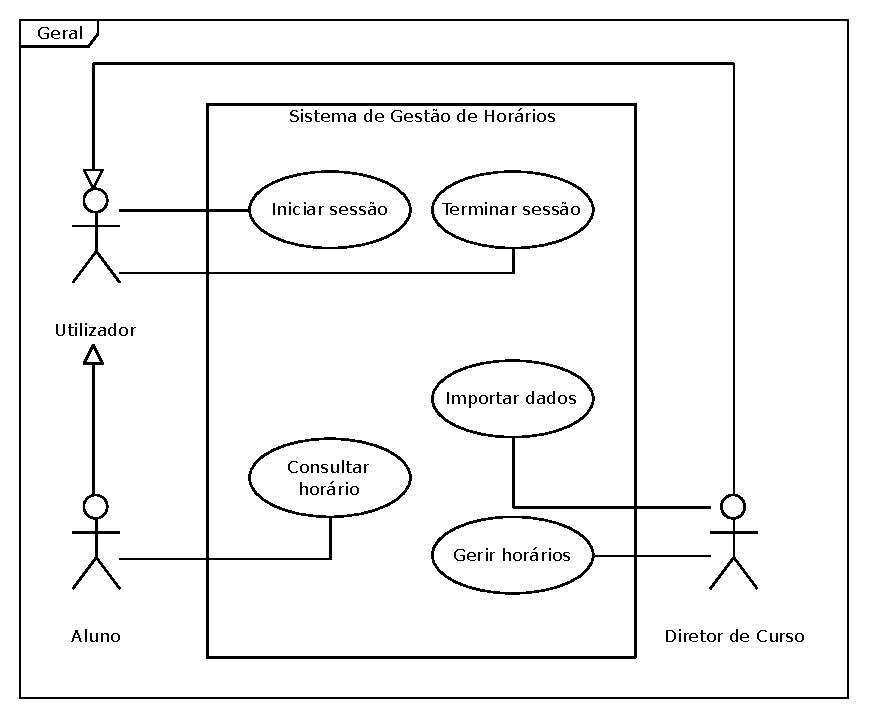
\includegraphics[width=0.6\textwidth]{Imagens/Modelos/UseCasesGeral.eps}
    \caption{Diagrama de casos de uso geral.}
\end{figure}

\begin{figure}[H]
    \centering
    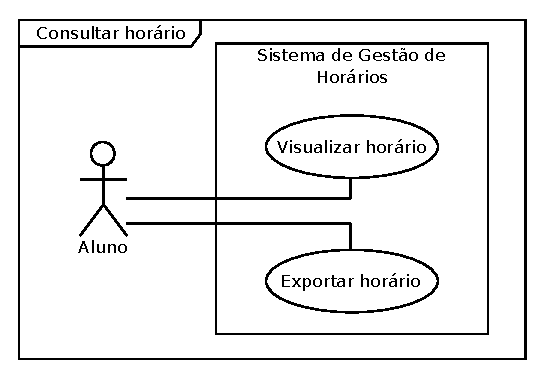
\includegraphics[width=0.6\textwidth]{Imagens/Modelos/UseCasesConsultarHorario.eps}
    \caption{Diagrama de casos de uso -- Consultar horário.}
\end{figure}

\begin{figure}[H]
    \centering
    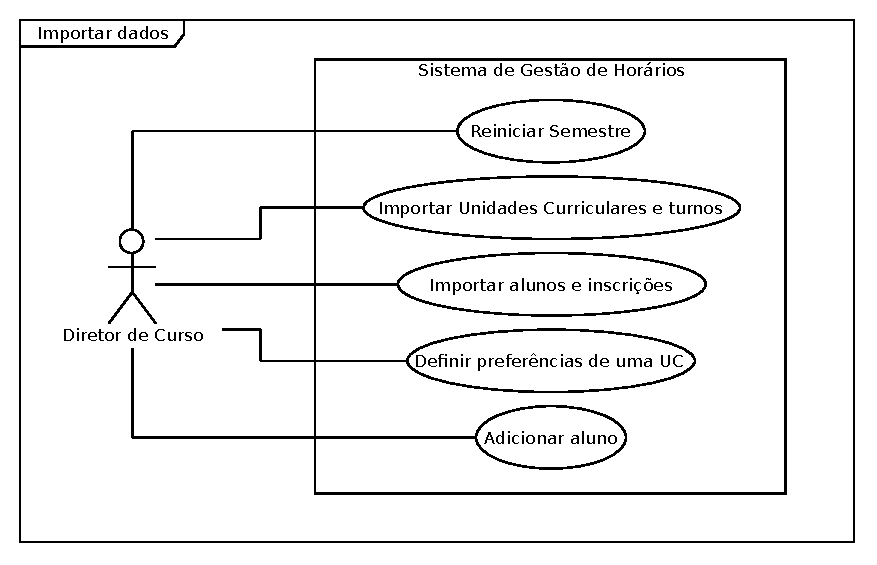
\includegraphics[width=0.6\textwidth]{Imagens/Modelos/UseCasesImportarDados.eps}
    \caption{Diagrama de casos de uso -- Importar dados.}
\end{figure}

\begin{figure}[H]
    \centering
    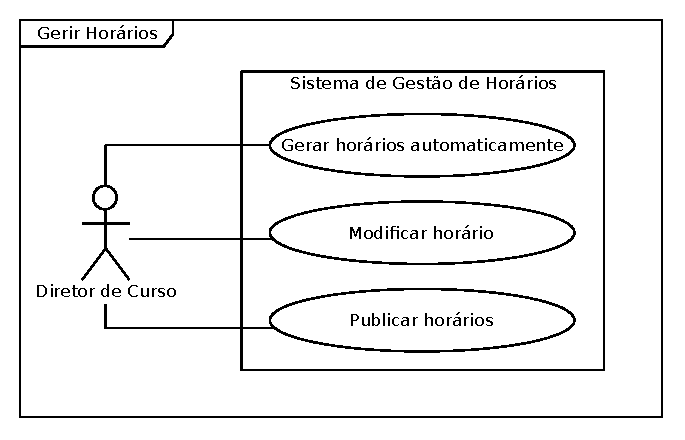
\includegraphics[width=0.6\textwidth]{Imagens/Modelos/UseCasesGerirHorarios.eps}
    \caption{Diagrama de casos de uso -- Gerir horários.}
\end{figure}

Note-se que há vários possíveis casos de uso que não foram considerados, nomeadamente casos de
uso relativos a operações CRUD de entidades como Alunos, Unidades Curriculares e Preferências de
UCs. A título de exemplo, o diretor de curso pode ter necessidade de adicionar novos alunos (este
\emph{use case} já se encontra definido), consultar os dados de um aluno existente, modificar os
dados de um aluno (por exemplo, por se encontrarem incorretos), ou remover um aluno do seu curso
(por exemplo, porque esse aluno pediu transferência de curso).

No entanto, como foi utilizada uma abordagem de desenvolvimento iterativa e incremental, nesta
primeira iteração apenas se pretende desenvolver um produto mínimo viável. Considerou-se que, nesta
iteração, o diretor de curso apenas seria capaz de importar dados em \emph{bulk}, sendo incapaz de
os consultar ou corrigir, mas capaz de adicionar novos alunos, caso surgissem novas inscrições após
o início do semestre. Ademais, considerou-se que a modificação manual de horários estaria
disponível, uma vez que esta é necessária para definir os horários dos alunos com estatuto e
corrigir problemas nos horários gerados automaticamente. Assim, a maior parte das operações CRUD
apenas serão consideradas em fases seguintes de desenvolvimento.

\subsection{Descrição dos Casos de Uso}

Seguem-se abaixo, as descrições dos casos de uso no modelo anteriormente apresentado.

\begin{usecase}
    {Iniciar sessão}
    {Ator autentica-se para poder realizar outras operações.}
    {Diretor de curso, Alunos}
    {\item Ator não tem sessão iniciada.}
    {\item Ator fica com sessão iniciada no sistema.}

    \flow{
        \item Ator indica o seu endereço de email e palavra-passe.
        \item Sistema valida o endereço de email e a palavra-passe.
        \item Sistema inicia uma sessão para o ator.
        \item Sistema informa que a autenticação teve sucesso.
    }

    \otherflow{Fluxo de exceção 1}{[combinação de email e palavra-passe incorreta] (passo 2)}{
        \item[2.1.] Sistema informa que a autenticação não teve sucesso.
    }
\end{usecase}

\begin{usecase}
    {Terminar sessão}
    {Ator fecha sessão previamente iniciada.}
    {Diretor de curso, Alunos}
    {\item Ator tem sessão iniciada.}
    {\item A sessão iniciada pelo ator é terminada.}

    \flow{
        \item Ator solicita o término da sua sessão.
        \item Sistema fecha a sessão previamente iniciada.
        \item Sistema informa ator de que a sessão foi fechada com sucesso.
    }
\end{usecase}

\begin{usecase}
    {Visualizar horário}
    {Ator consulta os turnos nos quais se encontra inscrito.}
    {Alunos}
    {
        \item Ator tem sessão iniciada;
        \item O horário do ator está disponível para consulta (já foi publicado).
    }
    {\item O horário atribuído ao ator é-lhe apresentado.}

    \flow{
        \item Ator solicita a consulta do seu horário.
        \item Sistema apresenta o horário atribuído ao ator.
    }
\end{usecase}

\begin{usecase}
    {Exportar horário}
    {Ator gera um ficheiro com os turnos do seu horário.}
    {Alunos}
    {
        \item Ator tem sessão iniciada;
        \item O horário do ator está disponível para consulta (já foi publicado).
    }
    {\item É gerado um ficheiro com o horário do ator.}

    \flow{
        \item Ator solicita a exportação do seu horário para um ficheiro.
        \item Ator indica onde esse ficheiro deve ser gravado.
        \item Sistema exporta o horário do ator para o ficheiro pedido.
        \item Sistema informa ator de sucesso na operação de exportação.
    }
\end{usecase}

\begin{usecase}
    {Reiniciar semestre}
    {Ator elimina todos os dados associados ao curso que dirige, para os importar novamente.}
    {Diretor de curso}
    {\item Ator tem sessão iniciada;}
    {
        \item Não há dados de UCs, turnos, alunos, inscrições, preferências de UCs e horários
            associados ao curso dirigido pelo ator.
    }

    \flow{
        \item Ator solicita a eliminação de todos os dados relacionados com o curso que dirige.
        \item Sistema elimina todos os dados de UCs, turnos, alunos, inscrições, preferências de UCs
            e horários associados ao curso dirigido pelo ator.
        \item Sistema informa ator de sucesso na operação.
    }
\end{usecase}

\begin{usecase}
    {Importar Unidades Curriculares e turnos}
    {
        Ator carrega para o sistema um ficheiro com a lista de Unidades Curriculares e turnos do
        curso que dirige.
    }
    {Diretor de curso}
    {\item Ator tem sessão iniciada.}
    {
        \item Dados que o sistema tem sobre UCs e turnos do curso dirigido pelo ator são os do
            ficheiro fornecido.
    }

    \flow{
        \item Ator solicita a importação de um ficheiro com Unidades Curriculares e os seus turnos.
        \item Sistema confirma que não existem Unidades Curriculares e turnos no curso dirigido pelo
            ator.
        \item Sistema pede o ficheiro com os dados.
        \item Ator fornece o ficheiro com os dados.
        \item Sistema confirma que os dados no ficheiro são válidos, e compatíveis com os dados já
            presentes no sistema.
        \item Sistema substitui os dados que tem sobre UCs e turnos do curso dirigido pelo ator
            pelos dados no ficheiro fornecido.
        \item Sistema informa ator de sucesso na operação de importação.
    }

    \otherflow{Fluxo alternativo 1}{[existem UCs e turnos do curso que o ator dirige] (passo 2)}{
        \item[2.1.] Sistema pergunta se o ator deseja sobrescrever os dados existentes.
        \item[2.2.] Ator responde que sim.
        \item[2.3.] Regressa a 3.
    }

    \otherflow{Fluxo de exceção 2}{[ator responde que não] (passo 2.2)}{
        \item[2.2.1.] Sistema aborta a importação de dados, informando o ator.
    }

    \otherflow{Fluxo de exceção 3}
        {[dados inválidos ou incompatíveis com dados já no sistema] (passo 5)}{

        \item[5.1.] Sistema aborta a importação de dados, informando o ator.
    }
\end{usecase}

\begin{usecase}
    {Importar alunos e inscrições}
    {
        Ator carrega para o sistema um ficheiro com a lista de alunos do curso que dirige, e em que
        Unidades Curriculares estes se encontram inscritos.
    }
    {Diretor de curso}
    {
        \item Ator tem sessão iniciada;
        \item Existem UCs e turnos do curso dirigido pelo ator.
    }
    {
        \item Dados que o sistema tem sobre alunos e inscrições do curso dirigido pelo ator são os
            do ficheiro fornecido.
    }

    \flow{
        \item Ator solicita a importação de um ficheiro com alunos e as suas inscrições em UCs.
        \item Sistema confirma que não existem alunos e inscrições no curso dirigido pelo ator.
        \item Sistema pede o ficheiro com os dados.
        \item Ator fornece o ficheiro com os dados.
        \item Sistema confirma que os dados no ficheiro são válidos, e compatíveis com os dados
            presentes no sistema.
        \item Sistema gera uma palavra-passe e um horário vazio para cada aluno importado.
        \item Sistema substitui os dados que tem sobre alunos e inscrições do curso dirigido ator
            pelos dados no ficheiro fornecido.
        \item Sistema informa ator de sucesso na operação de importação.
    }

    \otherflow{Fluxo alternativo 1}
        {[existem alunos e inscrições em UCs do curso que o ator dirige] (passo 2)}{

        \item[2.1.] Sistema pergunta se o ator deseja sobrescrever os dados existentes.
        \item[2.2.] Ator responde que sim.
        \item[2.3.] Regressa a 3.
    }

    \otherflow{Fluxo de exceção 2}{[ator responde que não] (passo 2.2)}{
        \item[2.2.1.] Sistema aborta a importação de dados, informando o ator.
    }

    \otherflow{Fluxo de exceção 3}
        {[dados inválidos ou incompatíveis com dados já no sistema] (passo 5)}{

        \item[5.1.] Sistema aborta a importação de dados, informando o ator.
    }
\end{usecase}

\begin{usecase}
    {Definir preferências de uma UC}
    {
        Ator define, através de um ficheiro de dados, condições relativas a uma Unidade Curricular
        do curso que dirige, que devem ser respeitadas na geração automática de horários.
    }
    {Diretor de curso}
    {
        \item Ator tem sessão iniciada;
        \item Existem UCs e turnos do curso dirigido pelo ator.
    }
    {\item As preferências da UC escolhida pelo ator passam a ser as definidas pelo mesmo.}

    \flow{
        \item Ator indica que deseja definir as preferências de uma UC.
        \item Sistema apresenta a lista de Unidades Curriculares no curso dirigido pelo ator.
        \item Sistema pede ao ator que selecione uma Unidade Curricular.
        \item Ator seleciona uma Unidade Curricular.
        \item Sistema verifica que não existem já preferências para a Unidade Curricular
            selecionada.
        \item Sistema pede o ficheiro com as preferências.
        \item Ator fornece o ficheiro com as preferências.
        \item Sistema confirma que os dados no ficheiro são válidos, e compatíveis com os dados
            presentes no sistema.
        \item Sistema substitui as preferências da UC pelas fornecidas.
    }

    \otherflow{Fluxo alternativo 1}{[existem preferências para a UC selecionada] (passo 5)}{
        \item[5.1.] Sistema pergunta se o ator deseja sobrescrever os dados existentes.
        \item[5.2.] Ator responde que sim.
        \item[5.3.] Regressa a 6.
    }

    \otherflow{Fluxo de exceção 2}{[ator responde que não] (passo 5.2)}{
        \item[5.2.1.] Sistema aborta a importação de preferências, informando o ator.
    }

    \otherflow{Fluxo de exceção 3}
        {[dados inválidos ou incompatíveis com dados já no sistema] (passo 8)}{

        \item[8.1.] Sistema aborta a importação de preferências, informando o ator.
    }
\end{usecase}

\begin{usecase}
    {Adicionar aluno}
    {Ator adiciona um novo aluno matriculado no curso que dirige, juntamente com as UCs em que se
        encontra inscrito.}
    {Diretor de curso}
    {
        \item Ator tem sessão iniciada;
        \item Existem UCs e turnos no curso dirigido pelo ator.
    }
    {
        \item Aluno especificado pelo ator é registado como matriculado no curso dirigido pelo ator,
        juntamente com as UCs onde se encontra inscrito.
    }

    \flow{
        \item Ator solicita a adição um novo aluno.
        \item Sistema pede informação sobre o aluno: número de aluno, nome, endereço eletrónico,
            média de curso (se aplicável), se este tem estatuto, e a que este se deve.
        \item Ator insere a informação do aluno pedida.
        \item Sistema verifica que não tem registo desse aluno.
        \item Sistema apresenta lista de Unidades Curriculares do curso que o ator dirige.
        \item Sistema pede lista de Unidades Curriculares nas quais o aluno se encontra inscrito.
        \item Ator indica lista de Unidades Curriculares.
        \item Sistema gera uma palavra-passe e um horário vazio para o aluno.
        \item Sistema regista aluno como inscrito no curso dirigido pelo ator, e as UCs em que se
            encontra inscrito.
    }

    \otherflow{Fluxo de exceção 1}
        {[aluno com o mesmo número já existe] (passo 4)}{

        \item[4.1.] Sistema aborta a operação, informando o ator.
    }
\end{usecase}

\begin{usecase}
    {Gerar horários automaticamente}
    {
        Ator pede que o sistema automaticamente atribua turnos aos alunos do curso que dirige,
        atribuição esta que deve respeitar condições específicas bem definidas.
    }
    {Diretor de curso}
    {
        \item Ator tem sessão iniciada;
        \item Existem UCs e turnos no curso dirigido pelo ator;
        \item Existem alunos e inscrições no curso dirigido pelo ator.
    }
    {
        \item Cada aluno no curso dirigido pelo ator tem um horário atribuído, que ainda não pode
            consultar;
        \item Os horários gerados são constituídos pelos turnos que cada aluno precisa de frequentar
            (ex.: um aluno inscrito em DSS deve ter no seu horário um turno prático e um turno
             teórico dessa UC);
        \item Os horários gerados não contêm sobreposições de turnos;
        \item Os horários gerados respeitam os limites de inscrições nos turnos;
        \item Os horários gerados respeitam as preferências de distribuição dos regentes das UCs.
    }

    \flow{
        \item Ator solicita a geração automática de horários.
        \item Sistema gera horários, inteligentemente atribuindo turnos aos alunos do curso
            dirigido pelo ator, de modo a respeitar a pós-condição.
        \item Sistema armazena os horários gerados, ainda como não disponíveis para consulta pelos
            alunos.
        \item Sistema informa ator de sucesso na geração de horários.
    }

    \otherflow{Fluxo de exceção 1}
        {[não foi encontrada solução, em tempo útil, que respeite a pós-condição] (passo 2)}{

        \item[2.1.] Sistema armazena os horários gerados (apesar de imperfeitos), ainda como não
            disponíveis para consulta pelos alunos.
        \item[2.2.] Sistema procura violações da pós-condição nos horários gerados.
        \item[2.3.] Sistema informa ator de insucesso na geração de horários, e apresenta as
            violações encotradas ao ator.
    }
\end{usecase}

\begin{usecase}
    {Modificar Horário}
    {Ator altera que turnos estão e não estão presentes no horário de um aluno.}
    {Diretor de curso}
    {
        \item Ator tem sessão iniciada;
        \item Existem UCs e turnos no curso dirigido pelo ator;
        \item Existem alunos e inscrições no curso dirigido pelo ator.
    }
    {
        \item Horário do aluno passa a ser constituído pelos turnos indicados pelo ator.
        \item Os horário modificado é constituído pelos turnos que o aluno precisa de frequentar:
        \item O horário modificado não contém sobreposições de turnos;
        \item O horário modificado não causa desrespeito pelos limites de inscrições nos turnos;
        \item O horário modificado não causa desrespeito pelas preferências de distribuição dos
            regentes das UCs.
    }

    \flow{
        \item Ator solicita a modificação do horário de um aluno.
        \item Sistema pede o número do aluno.
        \item Ator providencia número do aluno.
        \item Sistema procura horário de aluno com o número providenciado.
        \item Sistema apresenta lista de turnos nos quais o aluno se encontra inscrito.
        \item Ator modifica lista apresentada pelo sistema.
        \item Sistema verifica que o horário do aluno respeita a pós-condição.
        \item Sistema armazena horário modificado.
        \item Sistema informa ator de sucesso na operação.
    }

    \otherflow{Fluxo de exceção 1}{[aluno não encontrado no curso dirigido pelo ator] (passo 4)}{
        \item[4.1.] Sistema informa que o aluno não foi encontrado e cancela a operação.
    }

    \otherflow{Fluxo de exceção 2}{[horário não respeita a pós-condição] (passo 7)}{
        \item[7.1.] Sistema armazena horário modificado (apesar de imperfeito).
        \item[7.2.] Sistema informa o ator da pós-condição violada, mas que o horário foi
            armazenado.
    }
\end{usecase}

\begin{usecase}
    {Publicar horários}
    {Ator torna visíveis para os alunos os horários que construiu.}
    {Diretor de curso}
    {
        \item Ator tem sessão iniciada;
        \item Existem alunos e inscrições no curso dirigido pelo ator.
    }
    {
        \item Os horários construídos pelo ator são registados como disponíveis para consulta pelos
            alunos;
        \item Os alunos inscritos no curso dirigido pelo ator são informados por correio eletrónico
            dos novos horários.
    }

    \flow{
        \item Ator solicita a publicação dos horários que construiu.
        \item Sistema regista que os horários dos alunos inscritos no curso dirigido pelo ator podem
            ser consultados pelos mesmos.
        \item Sistema envia mensagens de correio eletrónico aos alunos cujos horários foram
            publicados, informando-os de tal, e contendo as suas palavras-passe.
    }

    \otherflow{Fluxo de exceção 1}{[pelo menos um e-mail não conseguiu ser enviado] (passo 3)}{
        \item[3.1.] Sistema informa quais as mensagens de correio eletrónico que não puderam ser
            enviadas.
    }
\end{usecase}

\section{Diagrama de componentes}

\begingroup
    \newgeometry{left=1cm,bottom=1cm,right=1cm,top=1cm}
    \begin{landscape}
        \thispagestyle{empty}

        \begin{figure}
            \centering
            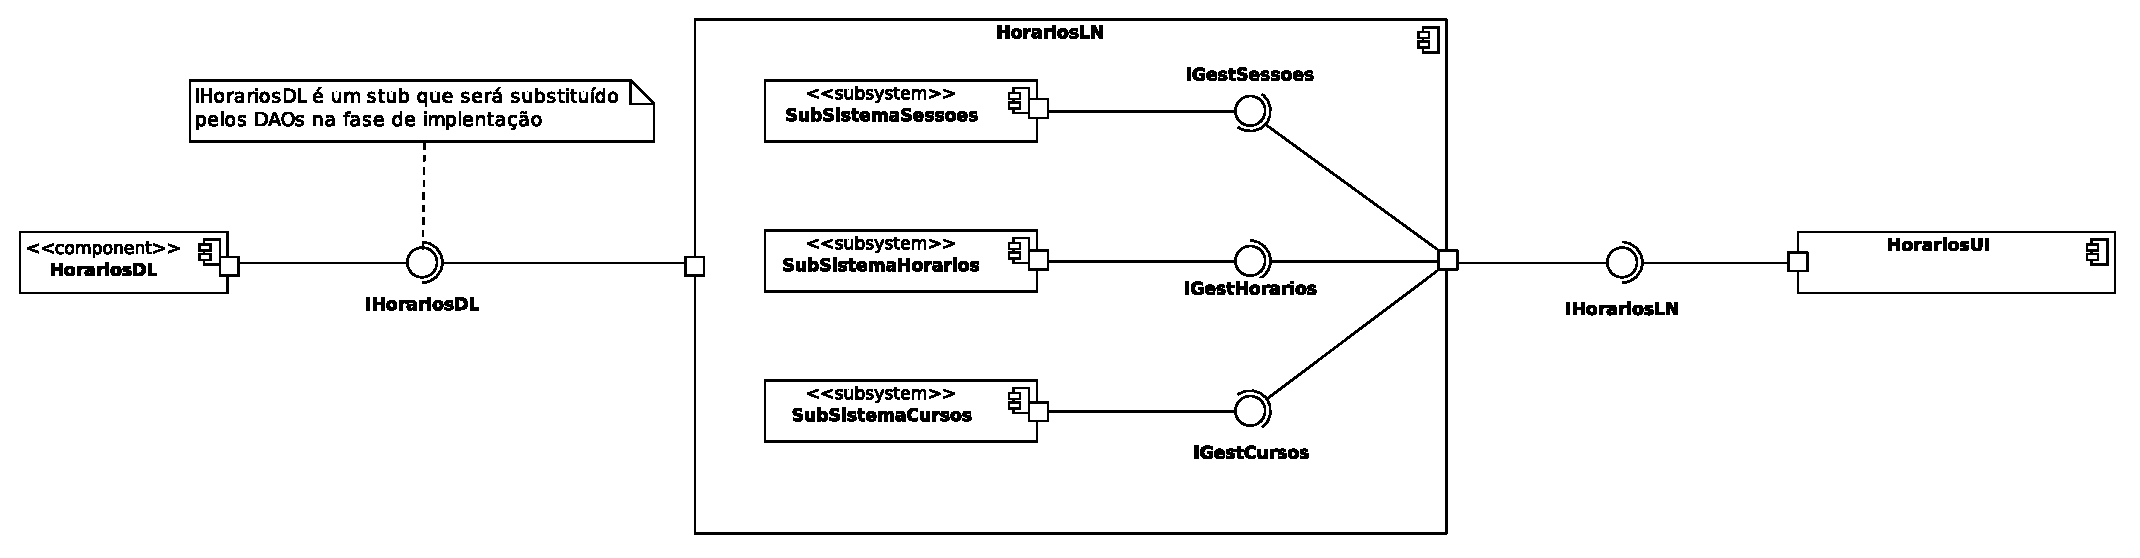
\includegraphics[scale=0.7]{Imagens/Modelos/Componentes.eps}
            \caption{
                Diagrama de componentes com uma visão de alto nível da arquitetura da aplicação.
            }
        \end{figure}
    \end{landscape}
\endgroup

\section{Anexos}

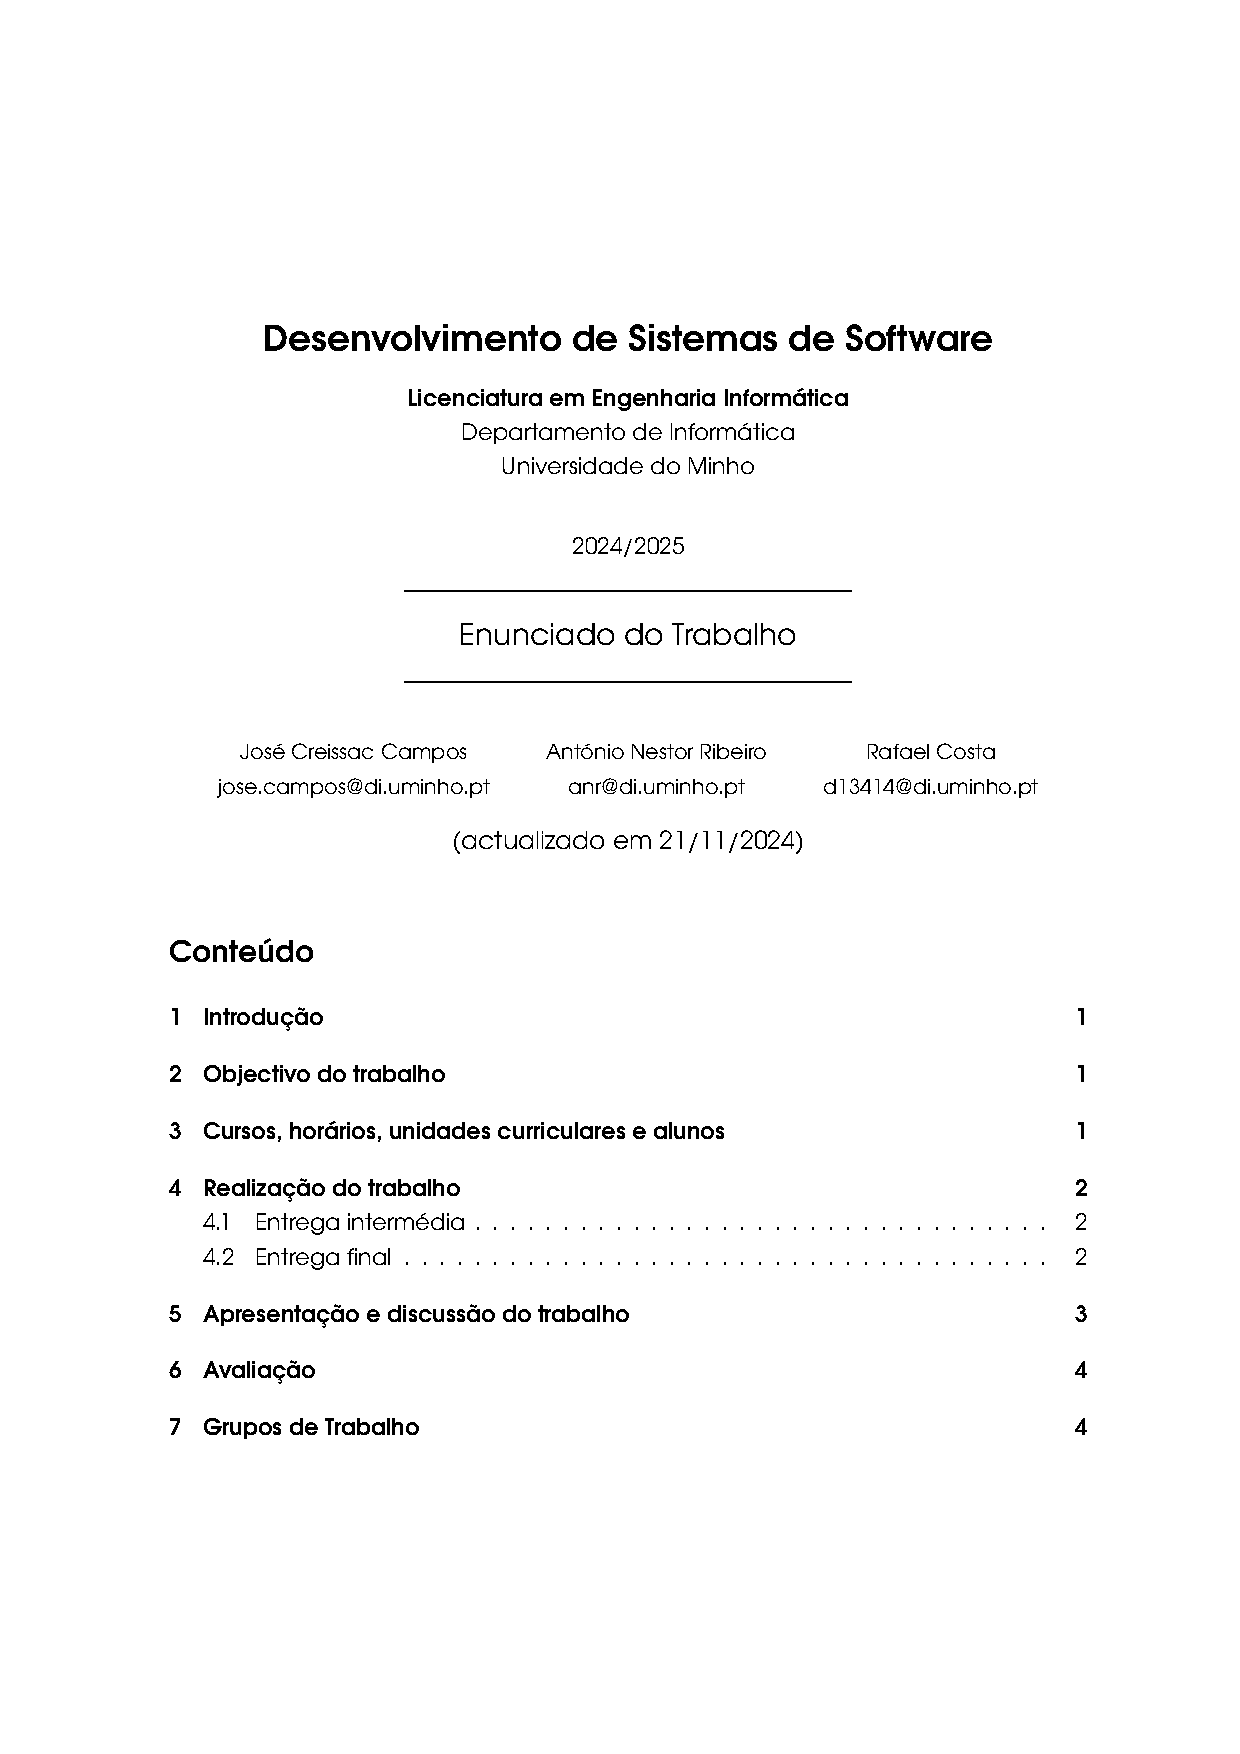
\includepdf[pages=1,pagecommand=\subsection{Enunciado do Trabalho}\thispagestyle{empty}]
    {../Enunciado.pdf}
\includepdf[pages=2-]{../Enunciado.pdf}

\subsection{Cenários}
\label{use-cases}

\textbf{O Diretor de Curso}

Após ter obtido a lista de alunos inscritos às UC do curso, através da Intranet, o diretor de curso
acedeu à aplicação de gestão de turnos e, depois de se ter autenticado, importou a lista de alunos
para o sistema. Como já anteriormente tinha importado a lista de UC e os seus horários, ficou em
condições de iniciar a geração dos horários dos alunos. Antes de o fazer, no entanto, definiu as
preferências que tinha recebidos dos docentes de algumas UC.

Uma das UC pediu que os alunos repetentes fossem colocados em turnos distintos dos alunos de
primeira inscrição para poder aplicar um método de ensino diferenciado. Uma outra enviou os grupos
de trabalho e pediu que os elementos de cada grupo ficassem no mesmo turno PL. Ainda uma outra,
pediu que os alunos fossem distribuídos pelos turnos de modo que ficassem agrupados por proximidade
da média de curso (uma forma de procurar ter turmas mais homogéneas). Finalmente, várias UC
definiram tamanhos máximos para os turnos TP/PL, diferentes do valor por omissão usado no curso.

Após configurar as preferências das UC, o diretor de curso pediu ao sistema uma primeira alocação
dos alunos aos turnos. O sistema realizou essa alocação, mas foi incapaz de colocar 45 alunos, por
não conseguir respeitar todas as preferências sem evitar conflitos nos seus horários.

O diretor de curso procedeu então à alocação manual desses alunos aos turnos disponíveis. Em alguns
casos o sistema avisou-o de conflitos nos horários dos alunos (ou no cumprimento das preferências
das UC). Na impossibilidade de evitar alguns desses conflitos, o diretor de curso optou por dar
prioridade aos alunos de primeira inscrição, fazendo a distribuição manual de modo a evitar
conflitos a esses alunos.

Após terminar a distribuição, o diretor de curso publicou os horários dos alunos.

\textbf{Os alunos}

A Maria recebeu uma notificação por email de que o seu horário tinha sido publicado. Acedeu à sua
versão da aplicação de gestão de turnos, consultou o horário e aproveitou para o exportar para a
sua agenda.

\end{document}
